\documentclass[border=4pt]{standalone}
\usepackage{amsmath,amssymb}
\usepackage{tikz}
\begin{document}
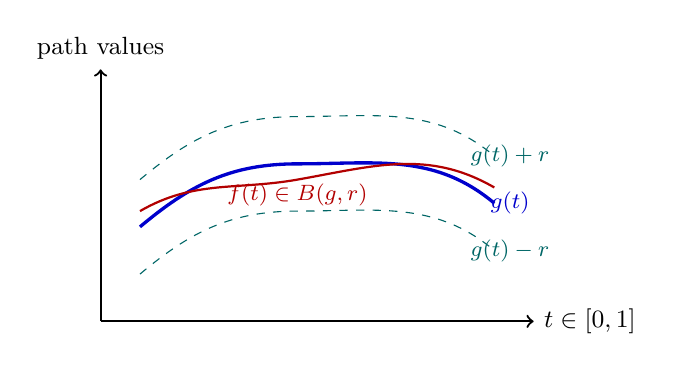
\begin{tikzpicture}[font=\small]
  \draw[->, thick] (0,0) -- (5.5,0) node[right] {$t \in [0,1]$};
  \draw[->, thick] (0,0) -- (0,3.2) node[above] {path values};

  % Center path g(t)
  \draw[very thick, blue!80!black] (0.5, 1.2) to[out=40, in=180] (2.5, 2.0) to[out=0, in=140] (5.0, 1.5);
  \node[blue!80!black, font=\footnotesize] at (5.2, 1.5) {$g(t)$};

  % Upper envelope g(t) + r
  \draw[dashed, teal!80!black] (0.5, 1.8) to[out=40, in=180] (2.5, 2.6) to[out=0, in=140] (5.0, 2.1);
  \node[teal!80!black, font=\footnotesize] at (5.2, 2.1) {$g(t)+r$};

  % Lower envelope g(t) - r
  \draw[dashed, teal!80!black] (0.5, 0.6) to[out=40, in=180] (2.5, 1.4) to[out=0, in=140] (5.0, 0.9);
  \node[teal!80!black, font=\footnotesize] at (5.2, 0.9) {$g(t)-r$};

  % Perturbed path f(t) inside tube
  \draw[thick, red!70!black] (0.5, 1.4) to[out=30, in=190] (2.5, 1.8) to[out=10, in=150] (5.0, 1.7);
  \node[red!70!black, font=\footnotesize] at (2.5, 1.6) {$f(t) \in B(g,r)$};
\end{tikzpicture}
\end{document}